\documentclass[10pt,a4paper,titlepage]{article}
\usepackage[utf8]{inputenc}
\usepackage{amsmath}
\usepackage{amsfonts}
\usepackage{amssymb}
\usepackage{graphicx}
\usepackage{lmodern}
\usepackage{xcolor}
\usepackage{qtree}
\usepackage{listings}
\usepackage{color}
\usepackage[xetex, hypertexnames=false, breaklinks=true, pdfborder={0 0 0},
pdfauthor={Timo Homburg},
pdftitle={Quiz Projektbeschreibung},
pdfsubject={Quiz Projekt},
pdfkeywords={Java,Game,Quiz},
pdfproducer={Xetex with hyperref},
pdfcreator={Pdflatex}]{hyperref}
\definecolor{gray}{rgb}{0.4,0.4,0.4}
\definecolor{darkblue}{rgb}{0.0,0.0,0.6}
\definecolor{cyan}{rgb}{0.0,0.6,0.6}
\lstset{
	basicstyle=\footnotesize,
	frame=single,,
	columns=fullflexible,
	showstringspaces=false,
	commentstyle=\color{gray}\upshape,
	keepspaces
	% Linienstaerke des Rahmens
}
\lstdefinelanguage{XML}
{
	morestring=[b]",
	morestring=[s]{>}{<},
	morecomment=[s]{<?}{?>},
	stringstyle=\color{black},
	identifierstyle=\color{darkblue},
	keywordstyle=\color{cyan},
	morekeywords={xmlns,version,type}% list your attributes here
}
\begin{document}
	\tableofcontents
	\ \\\\\\\
	\textbf{\large Quiz Projektbeschreibung}\\
	\section{Einleitung}
	Ein Quiz mit 3 verschiedenen Fragetypen, Logbuch und 2P-Modus
	\section{Ziele und Features}
	Das Quiz bietet die Möglichkeit einen 1P-Modus zu starten (das normale Spiel).
	In der Standardeinstellung sind alle verfügbaren Fragetypen (Multiple Choice Frage, Freitextfrage und Bildfrage) aktiviert.
	Verfügbar sind die Fragetypen, welche bei Start des Programmes erfolgreich aus den vordefinierten XML-Dateien „multiplechoice.xml“,“imagequestion.xml“ und „freequestion.xml“ geladen wurden.
	War das Laden eines oder mehrerer Fragetypen bzw. einzelner Fragen nicht erfolgreich, so kann dies sowohl im Konsolenlog, also auch in der Datei „error.log“ nachvollzogen werden.
	Wird ein neues Spiel gestartet erfolgt eine Abfrage des Spielernamens.
	Anschließend wird mit einem Zufallswert wird nun ein Fragetyp ausgewählt und eine noch nicht richtig/falsch beantwortete Frage ausgewählt.
	Die Unterscheidung ob eine Frage noch nicht bzw. falsch beantwortet wurde erfolgt über die Speicherung jeder erfolgreich beantworteten Frage nach Fragetyp in einer Liste.
	Diese so eingetragenen Fragen sind von der Auswahl so lange ausgeschlossen bis alle anderen Fragen korrekt beantwortet wurden oder ein neues Spiel mit entsprechender Logeinstellung gestartet wird.
	Standardmäßig werden pro Spiel 10 Fragen gestellt.
	Nach der Beantwortung einer Frage erfolgt eine Benachrichtigung des Benutzers ob die Antwort richtig war. Bei Falschantwort erscheint zusätzlich eine Einblendung der richtigen Lösung.
	Anmerkung: Die Antworten der Freitextfragen sind unabhängig von Groß-und Kleinschreibung.
	Wird eine Frage richtig beantwortet erhöht sich außerdem der Punktezähler in der Statusleiste.
	Die Fragenanzahl pro Spiel kann im Einstellungsdialog den eigenen Wünschen angepasst werden.
	Sind alle Fragen gestellt erscheint im 1P-Modus die Anzahl der richtig beantworteten Fragen und die Gesamtanzahl der Fragen auf einem Beendigungsscreen.
\subsection{2 Spieler Modus}
Ist der 2P-Modus aktiv, so muss vor der Beantwortung einer Frage zunächst ein Button gedrückt werden.
Für Spieler 1 ist dies der Button STRG, für Spieler 2 der Button AltGr.
In der Statusleiste wird angezeigt welcher Spieler die Frage beantworten darf.
Erst danach hat einer der Spieler die Möglichkeit die jeweilige Frage zu beantworten.
Antwortet der jeweilige Spieler falsch, erhält sein Gegner einen Punkt.
Die Auswertung des 2P-Spiels auf dem Beendigungsscreen erfolgt über die Punkte:
Hierbei wird sowohl der Sieger ermittelt als auch ein Punkteergebnis dargestellt.
\subsection{Einstellungen}
Im Einstellungsdialog kann der User die o.g. Anzahl der Fragen pro Spiel anpassen.
Wird eine Fragenanzahlanpassung während einem laufenden Spiel durchgeführt, so hat dies unmittelbare Auswirkungen auf das Spiel wenn die neu eingetragene Fragenanzahl größer als die vorherige ist oder wenn die neue Fragenanzahl kleiner als die vorherige ist, jedoch das Spiel noch nicht bis zur letzten Frage (gerechnet von der neuen Fragenanzahl) fortgeschritten ist.
In allen anderen Fällen gilt die Wirksamkeit der neuen Fragenmengeneinstellung erst ab dem nächsten Spielbeginn.
Tritt die Einstellung nicht sofort in Kraft wird der Benutzer über den Umstand informiert.
Zusätzlich ist es möglich die 3 Fragetypen an und abzuschalten (sofern nicht alle 3 auf einmal abgeschaltet werden).
Die An/Abschaltoption ist jedoch abhängig von deren Verfügbarkeit und wirkt sich unmittelbar, auch auf ein gerade laufendes Spiel aus.
Ist ein bestimmter Fragetyp nicht verfügbar, so ist die zugehörige Checkbox nicht aktiviert. 
Konnten keine Fragetypen geladen werden, so erscheint eine Fehlermeldung bei Start eines neuen Spiels bzw. bei öffnen des Programmes.
Im Optionsdialog ist es zudem möglich einzustellen ob der Log der gestellten Fragen nach jeder Quizrunde gelöscht werden soll oder bis zur Beendigung des Programms bestehen soll.
Als weitere Optionen des Programmes existiert eine kleine Spielanleitung unter dem Menüpunkt „Manual“ und Programminformationen unter dem Button „About“.
\section{Programmarchitektur}
Wie im folgenden Klassendiagramm und in der Doxygen Dokumentation aufgeführt besteht das Programm aus verschiedenen Klassen die nun im einzelnen beschrieben werden sollen.
\begin{figure}
	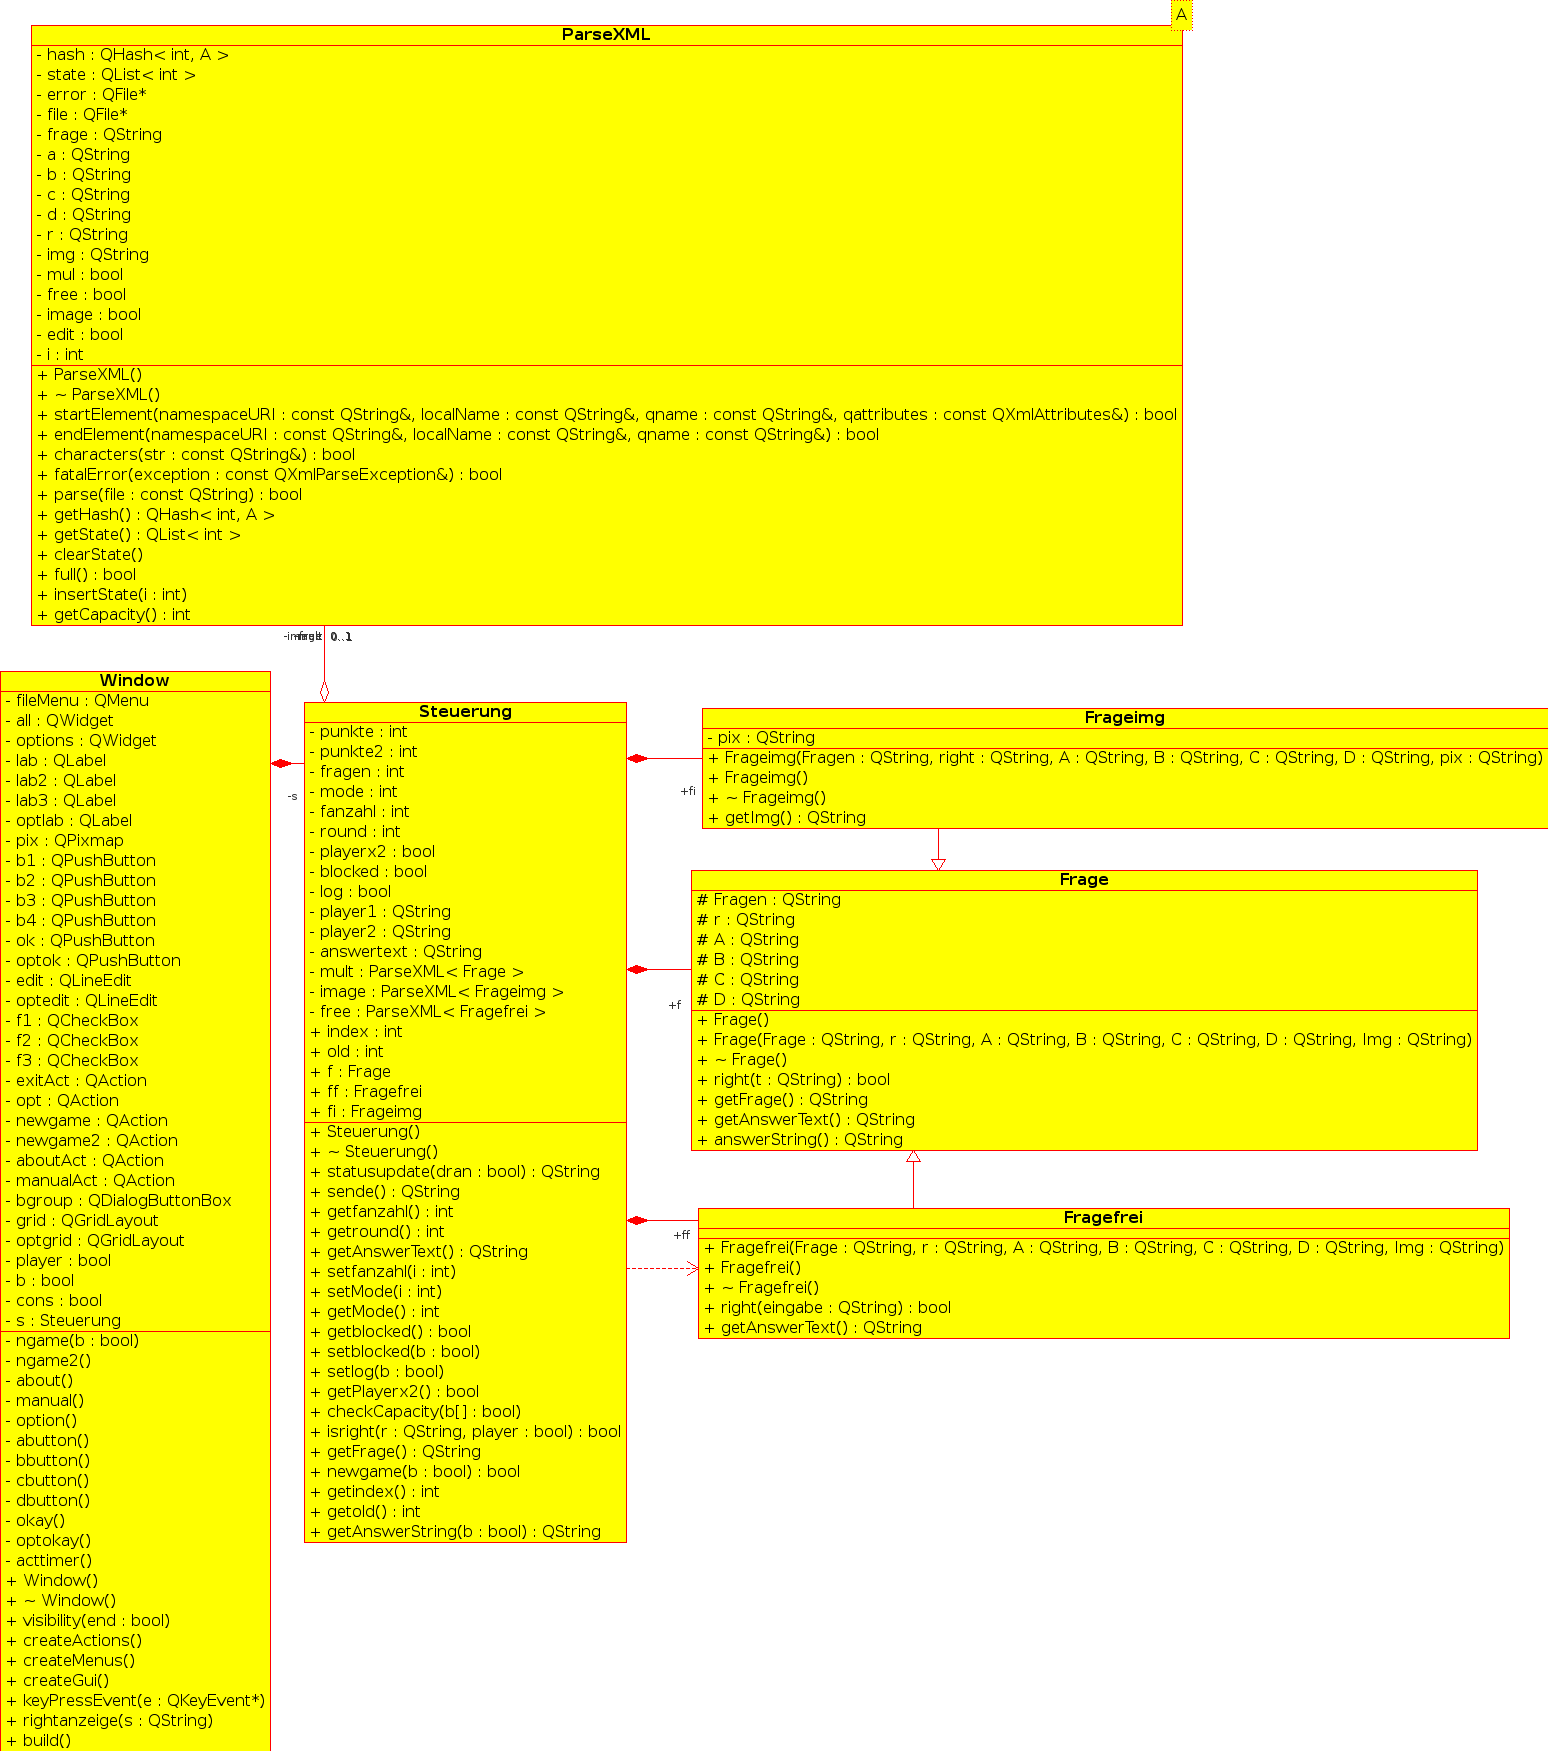
\includegraphics[width=\linewidth]{img/doku.png}
	\caption{Klassendiagramm}
\end{figure}
\begin{itemize}
	\item Die Klasse ParseXML ist eine generische Klasse, die das einlesen der verschiedenen XML-Dateien mit den Quizfragen ermöglicht.
	Sie erbt von der Klasse QXMLDefaultHandler und stellt somit selbst den Default und ErrorHandler für den zum Einlesen benutzten QXMLSimpleReader.
	Die Klasse übernimmt zudem die Ausgabe eventueller Fehler in den Errorlog bzw. die Konsole.
	In ParseXML existiert ein QHash zur Speicherung des aktuellen Fragetyps mit einem laufenden Index und eine Qlist zur Speicherung schon gestellter Fragen (bzw. deren Index) um das Logbuch für jeden Fragetyp zu realisieren.
	\item Benutzt wird die Klasse ParseXML von der Klasse Steuerung.
	Steuerung legt 3 ParseXML Objekte mit den unterschiedlichen zu parsenden Fragetypen an.
	Zudem kümmert sich die Klasse um die Verwaltung der zu speichernden Werte (z.B. Spielernamen, Punkteverteilungen u.ä.).
	Wichtige Funktionen die das Spiel steuern wie z.B. newgame() für ein neues Spiel, getFrage() um die nächste Frage auszuwählen oder isright() zur Prüfung auf Richtigkeit der gegebenen Antwort sind ebenfalls in dieser Klasse vorhanden.
	Die Verwaltung des Logs der in den ParseXML-Objekten gespeichert ist wird über Getter und Setter Funktionen von der Klasse Steuerung übernommen.
	Die Klasse bietet zudem Funktionalität zur Aufbereitung von Strings die im Fenster angezeigt werden.
	Beispiele hierfür sind die Funktion statusupdate() für die Statusleiste, oder getAnswerText() für die Zusammenstellung der richtigen Antwort bei falscher Antwort des Spielers.
	Implementiert ist auch eine Prüfungsfunktion zur Überprüfung ob überhaupt Fragen vorhanden sind.
	\item Eine Gruppe von Klassen sind die Fragenklassen.
	Die Oberklasse der Fragen ist die Klasse Frage.
	Diese repräsentiert die Multiple Choice Frage.
	In ihr befinden sich ein Qstring für die Frage, 4 Qstrings für die Antwortmöglichkeiten und ein Qstring für die richtige Antwort.
	Implementiert sind Funktionen zur Prüfung einer Antwort auf Richtigkeit und eine Funktion um die 4 Antwortmöglichkeiten in einen String für die Bildschirmausgabe zu schreiben.
	\item Von der Klasse Frage  erben die Unterklassen Fragefrei und Frageimg.
	Fragefrei implementiert hier nur eine andere Funktion für die Ausgabe des AnswerTextes.
	Frageimg erweitert die Klasse Frage um die Funktion getImg() um den Pfad des Bildes zurückzugeben und um den String Parameter für das Bild.
	\item Die Window Klasse erstellt das Hauptfenster, die Statusleiste, das Menü und seine Aktionen.
	Ebenfalls in dieser Klasse werden die Fenster des Optionsmenüs und das Manual sowie das Aboutfenster erstellt.
	Window erbt von der Klasse QMainWindow.
	Auch findet man in der Klasse Window die Umsetzung der verschiedenen für die Buttons und Menüs gebrauchten Signale und Slots.
	Es wird hierbei auf schon exisitierende Signale des QMainWindow zurückgegriffen und diese mit den in Klasse Window definierten Slots verknüpft.
	Ebenfalls in dieser Klasse enthalten ist der KeyListener für den 2P-Mode, der die Synchronisation der beiden Spieler regelt.
	Die Funktion Visibility ist zuständig für das Umschalten der Widgetelemente wenn die Fragen wechseln.
	In ihr werden auch eventuell nötige Bilder für die Bildfragen geladen.
	Die Funktion rightanzeige() stellt die richtige Antwort bzw. eine Bestätigung für eine korrekte Antworteingabe dar.
	\item In der Mainfunktion wird eine neue QApplication erstellt und das eventuell schon vorhandene Errorlogfile wird versucht zu löschen, damit es wenn nötig wieder neu beschrieben werden kann.
\end{itemize}
\section{Fehlerbehandlung}
Beim Parsen der XML-Files kann es verschiedene Fehler geben die hier im Einzelnen aufgeführt werden sollen:
Alle diese Fehler werden sowohl in der Error.Log Datei dokumentiert als auch in der Konsole ausgegeben.
\begin{itemize}
	\item Eine oder mehrere der 3 Dateien multiplechoice.xml, freequestion.xml und imagequestion.xml ist nicht vorhanden.
	\item Eine Frage konnte aufgrund fehlerhafter Parameter nicht eingelesen werden.
	\item Eine Frage konnte aufgrund fehlender Parameter nicht eingelesen werden.
	\item Der Pfad einer Bilddatei für die Bildfrage ist ungültig.
	\item Fehler die der QXMLSimpleReader aufgrund fehlerhafter XML-Syntax als Exception wirft.
\end{itemize}

Sollte aufgrund fehlender Schreibrechte oder anderen Exceptions die Datei error.log nicht erstellt werden können, so werden die Fehlermeldungen trotzdem in der Konsole ausgegeben und das Fehlen des Logfiles in der Konsole dokumentiert.

Fehler die der Benutzer als Fehlermeldungen im Programm angezeigt bekommt betreffen:
Einen Startversuch eines Quizspiels wenn keine Fragen vorhanden sind und die Auswahl keines Fragetypen im Optionsdialog oder die fehlende Eingabe der Frageanzahl im selbigen Dialog.
Zudem wird der Benutzer zusätzlich zu Beginn des Spiels wenn keine Fragen vorhanden sind über den Umstand informiert.

XML-Tags die nicht den folgenden 3 Tags entsprechen werden beim Parsen ignoriert.
Es entstehen hier also keine Fehlermeldungen.
\begin{lstlisting}[caption=Korrekte Tags]
<Multchoice A=“A“ B=“B“ C=“C“ D=“D“ Right=“A“>Frage</Multchoice>
<Image A=“A“ B=“B“ C=“C“ D=“D“ Right=“A“ Img=“Pfad“>Frage</Image>
<Fragefrei Right=“Antwort“>Frage</Fragefrei>
\end{lstlisting}
Es existieren 3 Demonstrationsfiles für die verschiedenen Fehlerfälle im Ordner errorxml.
Werden die 3 existierenden XML-Dateien durch diese ersetzt wird das Programm alle Fehlertypen ausgeben.
Zur Demonstration des Extremfalles können alle XML-Files verschoben werden.
\section{Anmerkungen und Erweiterungen}
Auf das Speichern der Einstellungen oder des „Spielstandes“ des Spieles in Form der Speicherung der schon gestellten Fragen in einer Konfigurationsdatei wurde bei dem Quizspiel verzichtet.
Es ergibt sich somit ein komplettes Reset der Einstellungen und der gestellten Fragen bei jedem Neustart des Spieles. Desweiteren kann in zukünftigen Versionen des Spiels ein Karteneditor und eine Übersetzung sowohl der Kartensets als auch der GUI angestrebt werden.
	
\end{document}